%%%%%%%%%%%%%%%%%%%%%%%%%%%%%%%%%%%%%%%%%%%%%%%%%%%%%%%%%%%%%%%%%%%%%
%% This is a (brief) model paper using the achemso class
%% The document class accepts keyval options, which should include
%% the target journal and optionally the manuscript type.
%%%%%%%%%%%%%%%%%%%%%%%%%%%%%%%%%%%%%%%%%%%%%%%%%%%%%%%%%%%%%%%%%%%%%
\documentclass[journal=jacsat,manuscript=article]{achemso}

%%%%%%%%%%%%%%%%%%%%%%%%%%%%%%%%%%%%%%%%%%%%%%%%%%%%%%%%%%%%%%%%%%%%%
%% Place any additional packages needed here.  Only include packages
%% which are essential, to avoid problems later. Do NOT use any
%% packages which require e-TeX (for example etoolbox): the e-TeX
%% extensions are not currently available on the ACS conversion
%% servers.
%%%%%%%%%%%%%%%%%%%%%%%%%%%%%%%%%%%%%%%%%%%%%%%%%%%%%%%%%%%%%%%%%%%%%
\usepackage[version=3]{mhchem} % Formula subscripts using \ce{}
\usepackage{amsmath}

%%%%%%%%%%%%%%%%%%%%%%%%%%%%%%%%%%%%%%%%%%%%%%%%%%%%%%%%%%%%%%%%%%%%%
%% If issues arise when submitting your manuscript, you may want to
%% un-comment the next line.  This provides information on the
%% version of every file you have used.
%%%%%%%%%%%%%%%%%%%%%%%%%%%%%%%%%%%%%%%%%%%%%%%%%%%%%%%%%%%%%%%%%%%%%
%%\listfiles

%%%%%%%%%%%%%%%%%%%%%%%%%%%%%%%%%%%%%%%%%%%%%%%%%%%%%%%%%%%%%%%%%%%%%
%% Place any additional macros here.  Please use \newcommand* where
%% possible, and avoid layout-changing macros (which are not used
%% when typesetting).
%%%%%%%%%%%%%%%%%%%%%%%%%%%%%%%%%%%%%%%%%%%%%%%%%%%%%%%%%%%%%%%%%%%%%
\newcommand*\mycommand[1]{\texttt{\emph{#1}}}

%%%%%%%%%%%%%%%%%%%%%%%%%%%%%%%%%%%%%%%%%%%%%%%%%%%%%%%%%%%%%%%%%%%%%
%% Meta-data block
%% ---------------
%% Each author should be given as a separate \author command.
%%
%% Corresponding authors should have an e-mail given after the author
%% name as an \email command. Phone and fax numbers can be given
%% using \phone and \fax, respectively; this information is optional.
%%
%% The affiliation of authors is given after the authors; each
%% \affiliation command applies to all preceding authors not already
%% assigned an affiliation.
%%
%% The affiliation takes an option argument for the short name.  This
%% will typically be something like "University of Somewhere".
%%
%% The \altaffiliation macro should be used for new address, etc.
%% On the other hand, \alsoaffiliation is used on a per author basis
%% when authors are associated with multiple institutions.
%%%%%%%%%%%%%%%%%%%%%%%%%%%%%%%%%%%%%%%%%%%%%%%%%%%%%%%%%%%%%%%%%%%%%
\author{Elliott Capek}
\affiliation{Department of Biochemistry, Oregon State University}
\email{capeke@oregonstate.edu}
\phone{(971) 207 8193}
\author{Hassan Alnatah}
\author{Laikana Ly}
\author{Joey Orton}
%% \alsoaffiliation[]{}
\author{Aidan Estelle}
%% \affiliation{Department of Biochemistry, Oregon State University}

%%%%%%%%%%%%%%%%%%%%%%%%%%%%%%%%%%%%%%%%%%%%%%%%%%%%%%%%%%%%%%%%%%%%%
%% The document title should be given as usual. Some journals require
%% a running title from the author: this should be supplied as an
%% optional argument to \title.
%%%%%%%%%%%%%%%%%%%%%%%%%%%%%%%%%%%%%%%%%%%%%%%%%%%%%%%%%%%%%%%%%%%%%
\title[]{Click chemistry reveals an alternate mechanism for HPII catalase}

%%%%%%%%%%%%%%%%%%%%%%%%%%%%%%%%%%%%%%%%%%%%%%%%%%%%%%%%%%%%%%%%%%%%%
%% Some journals require a list of abbreviations or keywords to be
%% supplied. These should be set up here, and will be printed after
%% the title and author information, if needed.
%%%%%%%%%%%%%%%%%%%%%%%%%%%%%%%%%%%%%%%%%%%%%%%%%%%%%%%%%%%%%%%%%%%%%
\keywords{Catalase, noncanonical amino acid, active site, channel flow}

\begin{document}
%%%%%%%%%%%%%%%%%%%%%%%%%%%%%%%%%%%%%%%%%%%%%%%%%%%%%%%%%%%%%%%%%%%%%
%% The manuscript does not need to include \maketitle, which is
%% executed automatically.  The document should begin with an
%% abstract, if appropriate.  If one is given and should not be, the
%% contents will be gobbled.
%%%%%%%%%%%%%%%%%%%%%%%%%%%%%%%%%%%%%%%%%%%%%%%%%%%%%%%%%%%%%%%%%%%%%
\begin{abstract}
  %% This is an example document for the \textsf{achemso} document
  %% class, intended for submissions to the American Chemical Society
  %% for publication. The class is based on the standard \LaTeXe\
  %% \textsf{report} file, and does not seek to reproduce the appearance
  %% of a published paper.

  %% This is an abstract for the \textsf{achemso} document class
  %% demonstration document.  An abstract is only allowed for certain
  %% manuscript types.  The selection of \texttt{journal} and
  %% \texttt{manuscript} will determine if an abstract is valid.  If
  %% not, the class will issue an appropriate error.
  Abstract abstract abstracts abstract. Abstract abstract abstracts abstract. Abstract abstract abstracts abstract. Abstract abstract abstracts abstract. Abstract abstract abstracts abstract. Abstract abstract abstracts abstract. Abstract abstract abstracts abstract. Abstract abstract abstracts abstract.\\
\end{abstract}

%%%%%%%%%%%%%%%%%%%%%%%%%%%%%%%%%%%%%%%%%%%%%%%%%%%%%%%%%%%%%%%%%%%%%
%% Start the main part of the manuscript here.
%%%%%%%%%%%%%%%%%%%%%%%%%%%%%%%%%%%%%%%%%%%%%%%%%%%%%%%%%%%%%%%%%%%%%
\section{Introduction}
Catalase is an enzyme which catalyzes the reaction $2H_2O_2 \rightarrow O_2 + 2H_2O$. This is an important detoxification reaction, since hydrogen peroxide is a reactive toxin generated by several biological processes. Catalase is a tetrameric protein which uses a heme group in its active site to facilitate the breakdown of hydrogen peroxide. It is a unique protein in that its reaction evolves gas, and thus its activity can be seen with the bare eye. The protein has been studied as a target for tumor suppression drugs \cite{bauer}. The enzyme is also useful industrially, in particular in the bleaching of textiles \cite{amorim}.

The molecular mechaninism of catalase proceeds in two steps. First, the heme reduces a hydrogen peroxide, producing water and the so-called Cpd I. Then Cpd I oxidizes a second hydrogen peroxide, producing water and oxygen gas. This second step is mediated by a histidine near the active site \cite{alfonso-prieto}.

This bimolecular substrate mechanism relies on the efficient transport of hydrogen peroxide into the deeply buried active site. This is believed to be aided by an electrical gradient over 12 \AA between an active site aspartic acid and the positive heme iron \cite{chelikani}. Mutagenisis of this Asp to positive residues decreases activity up to 90\% \cite{chelikani}. However, this study was accomplished using only a few canonical amino acid substitutions, and provides relatively weak evidence for the electric field hypothesis.

In this study we seek to use the technique of bioorthogonal ligation to study the electric field hypothesis of catalase substrate transport. We will incorporate the noncanonical amino acid 3-nitrotyrosine into the active site, then use click chemistry to insert a gradient of charged particles into the active site. By using a large number of particles with charges varying from positive to negative, we can average out the effects of steric bulk and isolate the effect of field strength. The results of such a study would conclusively determine the importance of an electric field in the catalase active site.\\

\section{Methods}
\textbf{Protein expression}\\
Wildtype protein was expressed by transforming the plasmid pBad-HPII (Addgene ID 105839), containing WT HPII gene, into competent \textit{E. coli} DH10B cells via heat-shock. pBad-HPII plasmid includes ampicillin resistance, an imidazole promoter, and a 6xHis tag on the N-term of the HPII gene. Cells were then grown in autoinduction media with an arabinose inducer (0.1\% aspartate pH 7.5, 0.2\% glycerol, 100$\mu g / mL$ ampicillin, mineral salts, 0.05\% glucose, 20mM MgSO4, 0.05\% arabinose, trace metals and AA mix) for 48 hours, shaking, at 37C. Cells were then pelletized and stored at -80C.\\

The same protocol was followed for the ncAA mutant catalases F206NY and F206pAzF, except protein plasmid pBad-HPII TAG206 (Addgene ID 105846) was used as a base. ncAA translation machinery plasmids pDule-3-nitrotyrosine (Addgene ID 85498) and pDule-pCNF (85494), which contain a tetracycline resistance gene, a TAG tRNA, and a compatible tRNA synthase, were co-transformed into DH10B along with pBAD-HPII TAG206 for respective F206NY and F206pAzF cell lines. ncAA autoinduction media was supplemented with $25\mu g / mL$ tetracycline to select for both plasmids.\\

OD600 measurements of cultures at 48h growth time were 0.65, 0.58 and 0.45 arb. units for WT, F206NY and F206pAzF cells.\\

\textbf{Protein purification}\\
Pelletized cells were reconstituted in TALON equilibration buffer (50mM sodium phosphate, 300mM NaCl) and microfluidized, also in equilibration buffer. Lysed cells were spun down at 15K RPM for 20 minutes at 4C. Supernatant was collected and combined with 300$\mu L$ bed volume TALON beads per 100mL cultured cells. TALON-supernatant mix was nutated for 30 minutes at 4C. Bound beads were then spun down at 500g for 5 minutes and the supernatant discarded. The beads were applied to a pre-washed gravity-flow column at RT and washed twice with 10mL equilibration buffer. Elution was done using 2mL elution buffer (50mM sodium phosphate, 300mM NaCl, 250mM imidazole) into four 500$\mu L$ aliquots. Protein was then stored at 4C.\\

\textbf{Bradford assay}\\
A Bio-Rad Bradford assay kit was used using the standard protocol. Bovine serum albumin was used as the reference protein to construct the standard curve. Concentrations from 125 $\mu g / mL$ to 2 mg/mL were explored. Samples were incubated with dye in cuvettes for 5 minutes at RT. Samples were then analyzed via spectrophotometer at 595 \textit{nm} and used to create the standard curve shown in Figure \ref{fig:bradford-assay}. Protein samples were then compared to this standard curve to estimate their concentration.\\

\textbf{Qualitative activity assay}\\
10 $\mu g$ purified WT catalase was added to a 5\% solution of hydrogen peroxide in water. The mixture was then examined for bubble formation.\\

\section{Results}
DH10B cell lines with appropriate plasmids were grown for 48h and pelletized. Wildtype HPII-containing cells were purified using TALON resin. Purified wildtype protein and ncAA cell lysates are shown in Figure \ref{fig:pure-gel}. The expected band corresponding to an 84-kD protein is seen across all lanes, indicating the presence of a catalase single subunit in each cell line. Contaminant bands in the gel are very faint, indicating pure protein.\\

A Bradford assay of wildtype purified protein was then conducted. The results, shown in Figure \ref{fig:bradford-assay}, further verify the presence of protein in the purified sample.\\

A qualitative, rudimentary assay testing the activity of wildtype purified HPII catalase was conducted. This assay verified HPII-WT was active by producing bubbles.\\

\begin{figure}
\centering
\includegraphics[width=0.7\linewidth]{figures/pure-gel}
\caption{Electrophoresis gel of crude lysate and purified protein expression. Major band in purification lanes correspond to protein of approximately 80kD, as expected for a catalase single subunit. Crude negative control lanes lack 80kD band, consistent with noncanonical amino acid being necessary for noncanonical protein expression.}
\label{fig:pure-gel}
\end{figure}

\begin{figure}
  \centering
  \begin{minipage}{.4\textwidth}
    \begin{tabular}{lll}
      \hline
      Sample  & OD590 & mg/mL  \\
      \hline
      WT        & 2.18 & 2.74\\
      %% F206NY    & 0.71 & 0.83\\
      %% F206pAzF  & 1.51 & 1.88\\
      \hline
    \end{tabular}
  \end{minipage}
  \begin{minipage}{.59\textwidth}
    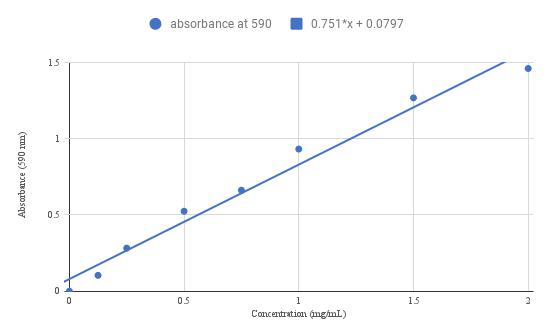
\includegraphics[width=\linewidth]{figures/bradford-standard-curve}
  \end{minipage}
  \caption{Bradford assay results. \textbf{Left:} Sample absorbance at 590 nm and extrapolated concentration. \textbf{Right:} Bradford standard curve.}
  \label{fig:bradford-assay}
\end{figure}

\subsection{References}

%%%%%%%%%%%%%%%%%%%%%%%%%%%%%%%%%%%%%%%%%%%%%%%%%%%%%%%%%%%%%%%%%%%%%
%% The same is true for Supporting Information, which should use the
%% suppinfo environment.
%%%%%%%%%%%%%%%%%%%%%%%%%%%%%%%%%%%%%%%%%%%%%%%%%%%%%%%%%%%%%%%%%%%%%
\begin{suppinfo}

\end{suppinfo}

%%%%%%%%%%%%%%%%%%%%%%%%%%%%%%%%%%%%%%%%%%%%%%%%%%%%%%%%%%%%%%%%%%%%%
%% The appropriate \bibliography command should be placed here.
%% Notice that the class file automatically sets \bibliographystyle
%% and also names the section correctly.
%%%%%%%%%%%%%%%%%%%%%%%%%%%%%%%%%%%%%%%%%%%%%%%%%%%%%%%%%%%%%%%%%%%%%
\bibliography{references}

%%%%%%%%%%%%%%%%%%%%%%%%%%%%%%%%%%%%%%%%%%%%%%%%%%%%%%%%%%%%%%%%%%%%%
%% The "tocentry" environment can be used to create an entry for the
%% graphical table of contents.
%%%%%%%%%%%%%%%%%%%%%%%%%%%%%%%%%%%%%%%%%%%%%%%%%%%%%%%%%%%%%%%%%%%%%

%% \begin{tocentry}

%% \end{tocentry}

\end{document}


results section mantra:
1 - Explain what you did and then describe what you expected as an outcome
2 - Describe the data and show the dta
3 - Interpret the data


Role of the lateral channel in catalase HPII of Escherichia coli, Loewen
They suggest that the perpendicular channel is the entrance channel and the lateral channel is the exhaust channel, because:
-enlarging the perpendicular channel increases peroxidatic activity
-perpendicular seems optimized for bringin in H2O2
-lateral channel is blocked in some catalases

Substrate Flow, Loewen
There are H2O2 binding sites in the heme distal pocket and main channel
There are several input channels; what are their purposes?
There is a ``molecular ruler'' in the main channel which selects for H2O2 against water
Active site mutations which allow more water in slow down the rxn rate
This paper discusses unidirectional flow of H2O2 through the main channel

Active and inhibited catalase structures, tainer
This is the paper about the hydrophobic ``molecular ruler''
A hydrophobic region distal to the heme cleft contains phenylalanines, tryptophan and two valines
Authors propose that two waters (one h-bonded to human Asn148 and His75; other h-bonded to gln168 and asp128) form a ``ruler''
This ``ruler'' is far enough apart that only H2O2 can stably occupy the distance betweeen, thus allowing only H2O2 to enter, not H2O
This would explain why opening the perpendicular channel decreases the rate
